\section{Data}
\label{sec:data}

Luminous red galaxies (LRGs) are massive galaxies that populate massive halos, lack active star formation, and are highly biased tracers of the dark matter gravitational field. A distinct break around 4000 \AA~in the LRG spectrum is often utilized to determine their redshifts accurately. LRGs are widely targeted in previous galaxy redshift surveys \citep[see, e.g.,][]{eisenstein2001spectroscopic, prakash2016sdss}, and their clustering and redshift properties are well studied \citep[see, e.g.,][]{ross2020MNRAS.498.2354R, gilmarin2020MNRAS.498.2492G, bautista2021MNRAS.500..736B, chapman2022MNRAS.516..617C}. 

DESI is designed to collect spectra of millions of LRGs covering the redshift range $0.2<z<1.35$. DESI selects its targets for spectroscopy from the DESI Legacy Imaging Surveys, which consist of three ground-based surveys that provide photometry of the sky in the optical $g$, $r$, and $z$ bands. These surveys include the Mayall $z$-band Legacy Survey using the Mayall telescope at Kitt Peak \citep[MzLS;][]{dey2018overview}, the Beijing–Arizona Sky Survey using the Bok telescope at Kitt Peak \citep[BASS;][]{zou2017project}, and the Dark Energy Camera Legacy Survey on the Blanco 4m telescope \citep[DECaLS;][]{flaugher2015dark}. As shown in Figure \ref{fig:ng}, the BASS and MzLS surveys observed the same footprint in the North Galactic Cap (NGC) while the DECaLS program observed both caps around the galactic plane; the BASS+MzLS footprint is separated from the DECaLS NGC at DEC $> 32.375$ degrees, although there is an overlap between the two regions for calibration purposes \citep{dey2018overview}. Additionally, the DECaLS program integrates observations executed from the Blanco instrument under the Dark Energy Survey \citep{abbott2016dark}, which cover about $1130 \deg^{2}$ of the South Galactic Cap (SGC) footprint. The DESI imaging catalogues also integrate the $3.4$ (W1) and $4.6$ $\mu m$ (W2) infrared photometry from the Wide-Field Infrared Explorer \citep[WISE;][]{wise2010AJ....140.1868W, meisner2018RNAAS...2....1M}.  


\subsection{DESI imaging LRGs}
Our sample of LRGs is drawn from the DESI Legacy Imaging Surveys Data Release 9 \citep[DR9;][]{dey2018overview} using the color-magnitude selection criteria designed for the DESI 1\% survey \mr{(CITE?)}, described as the Survey Validation 3 (SV3) selection in more detail in \cite{zhou2022target}. The color-magnitude selection cuts are defined in the $g$, $r$, $z$ bands in the optical and $W1$ band in the infrared, as summarized in Table \ref{tab:ts}. The selection cuts are developed differently for each imaging survey to reach an almost uniform target surface density, with an average density of $800$ galaxies per square degree covering around $18000$ square degrees, despite different survey efficiency and photometric calibration between DECaLS and BASS+MzLS. The implementation of these selection cuts in the DESI data processing pipeline is explained in \cite{myers2022}. The redshift distribution of our galaxy sample is inferred from DESI spectroscopy during the Survey Validation phase. A constant clustering amplitude is assumed for linear bias which is supported by \cite{zhou2021clustering}. Figure \ref{fig:nz} shows the redshift distribution (solid black line) and the evolution of linear bias (dashed red line) for our sample of LRGs.

\begin{figure}
 \centering
 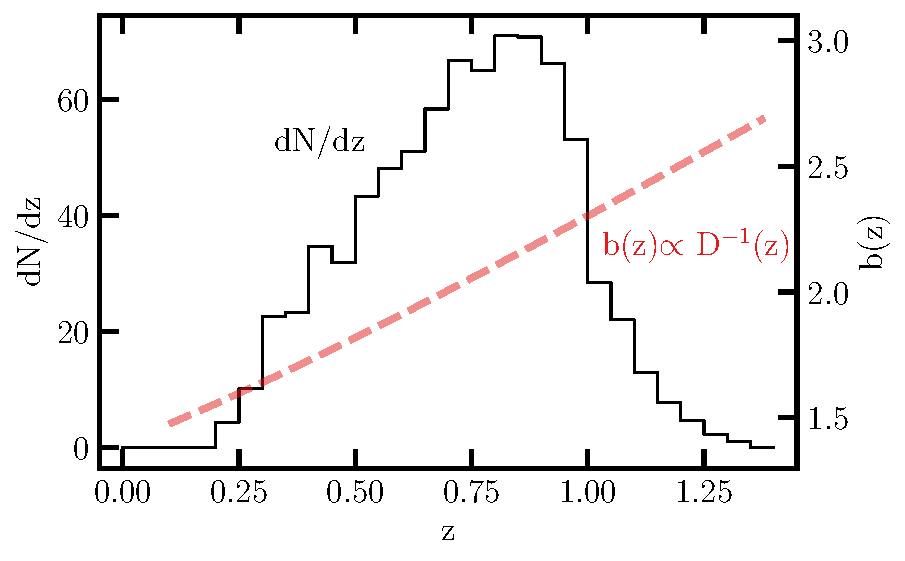
\includegraphics[width=0.45\textwidth]{figures/nz_lrg.pdf}
 \caption{The redshift distribution (solid line) and bias evolution (dashed line) of DESI LRG targets. The redshift distribution is determined by DESI spectroscopy. A constant clustering amplitude is assumed for linear bias, which determines the redshift evolution of bias by the growth factor $D(z)$.}
 \label{fig:nz}
\end{figure}

\begin{table*}
\caption{Selection criteria for the DESI-like LRG targets \citep{zhou2022target}. Magnitudes are corrected for Galactic extinction. $z_{\rm fiber}$ represents the z-band fiber magnitude, which corresponds to the expected flux within a DESI fiber.} \label{tab:ts}
 \centerline{%
 \begin{tabular}{lll}
 \hline
 \hline
 \textbf{Footprint} & \textbf{Criterion} &\textbf{Description}\\
 \hline
 \hline  
 & $z_{\rm fiber} < 21.7$ & Faint limit \\
  DECaLS & $z - W1 > 0.8 \times (r - z) - 0.6$ & Stellar rejection \\
 & $[(g-r >1.3)~{\rm AND}~((g-r) > -1.55*(r-W1) + 3.13)]~{\rm OR}~(r -W 1 > 1.8)$ & Remove low-z galaxies \\
 & $[(r-W1 > (W1 - 17.26)*1.8)~{\rm AND}~(r - W1 > W1 - 16.36)]~{\rm OR}~(r-W1 > 3.29)$ & Luminosity cut \\ 
 \hline
 & $z_{\rm fiber} < 21.71$ & Faint limit \\
 BASS+MzLS & $z - W1 > 0.8 \times (r - z) - 0.6$ & Stellar rejection \\
 & $[(g-r >1.34)~{\rm AND}~((g-r) > -1.55*(r-W1) + 3.23)]~{\rm OR}~(r -W 1 > 1.8)$ & Remove low-z galaxies \\
 & $[(r-W1 > (W1 - 17.24)*1.83)~{\rm AND}~(r - W1 > W1 - 16.33)]~{\rm OR}~(r-W1 > 3.39)$ & Luminosity cut \\ 
 \hline
 \end{tabular}}
\end{table*}

\begin{figure*}
 \centering
 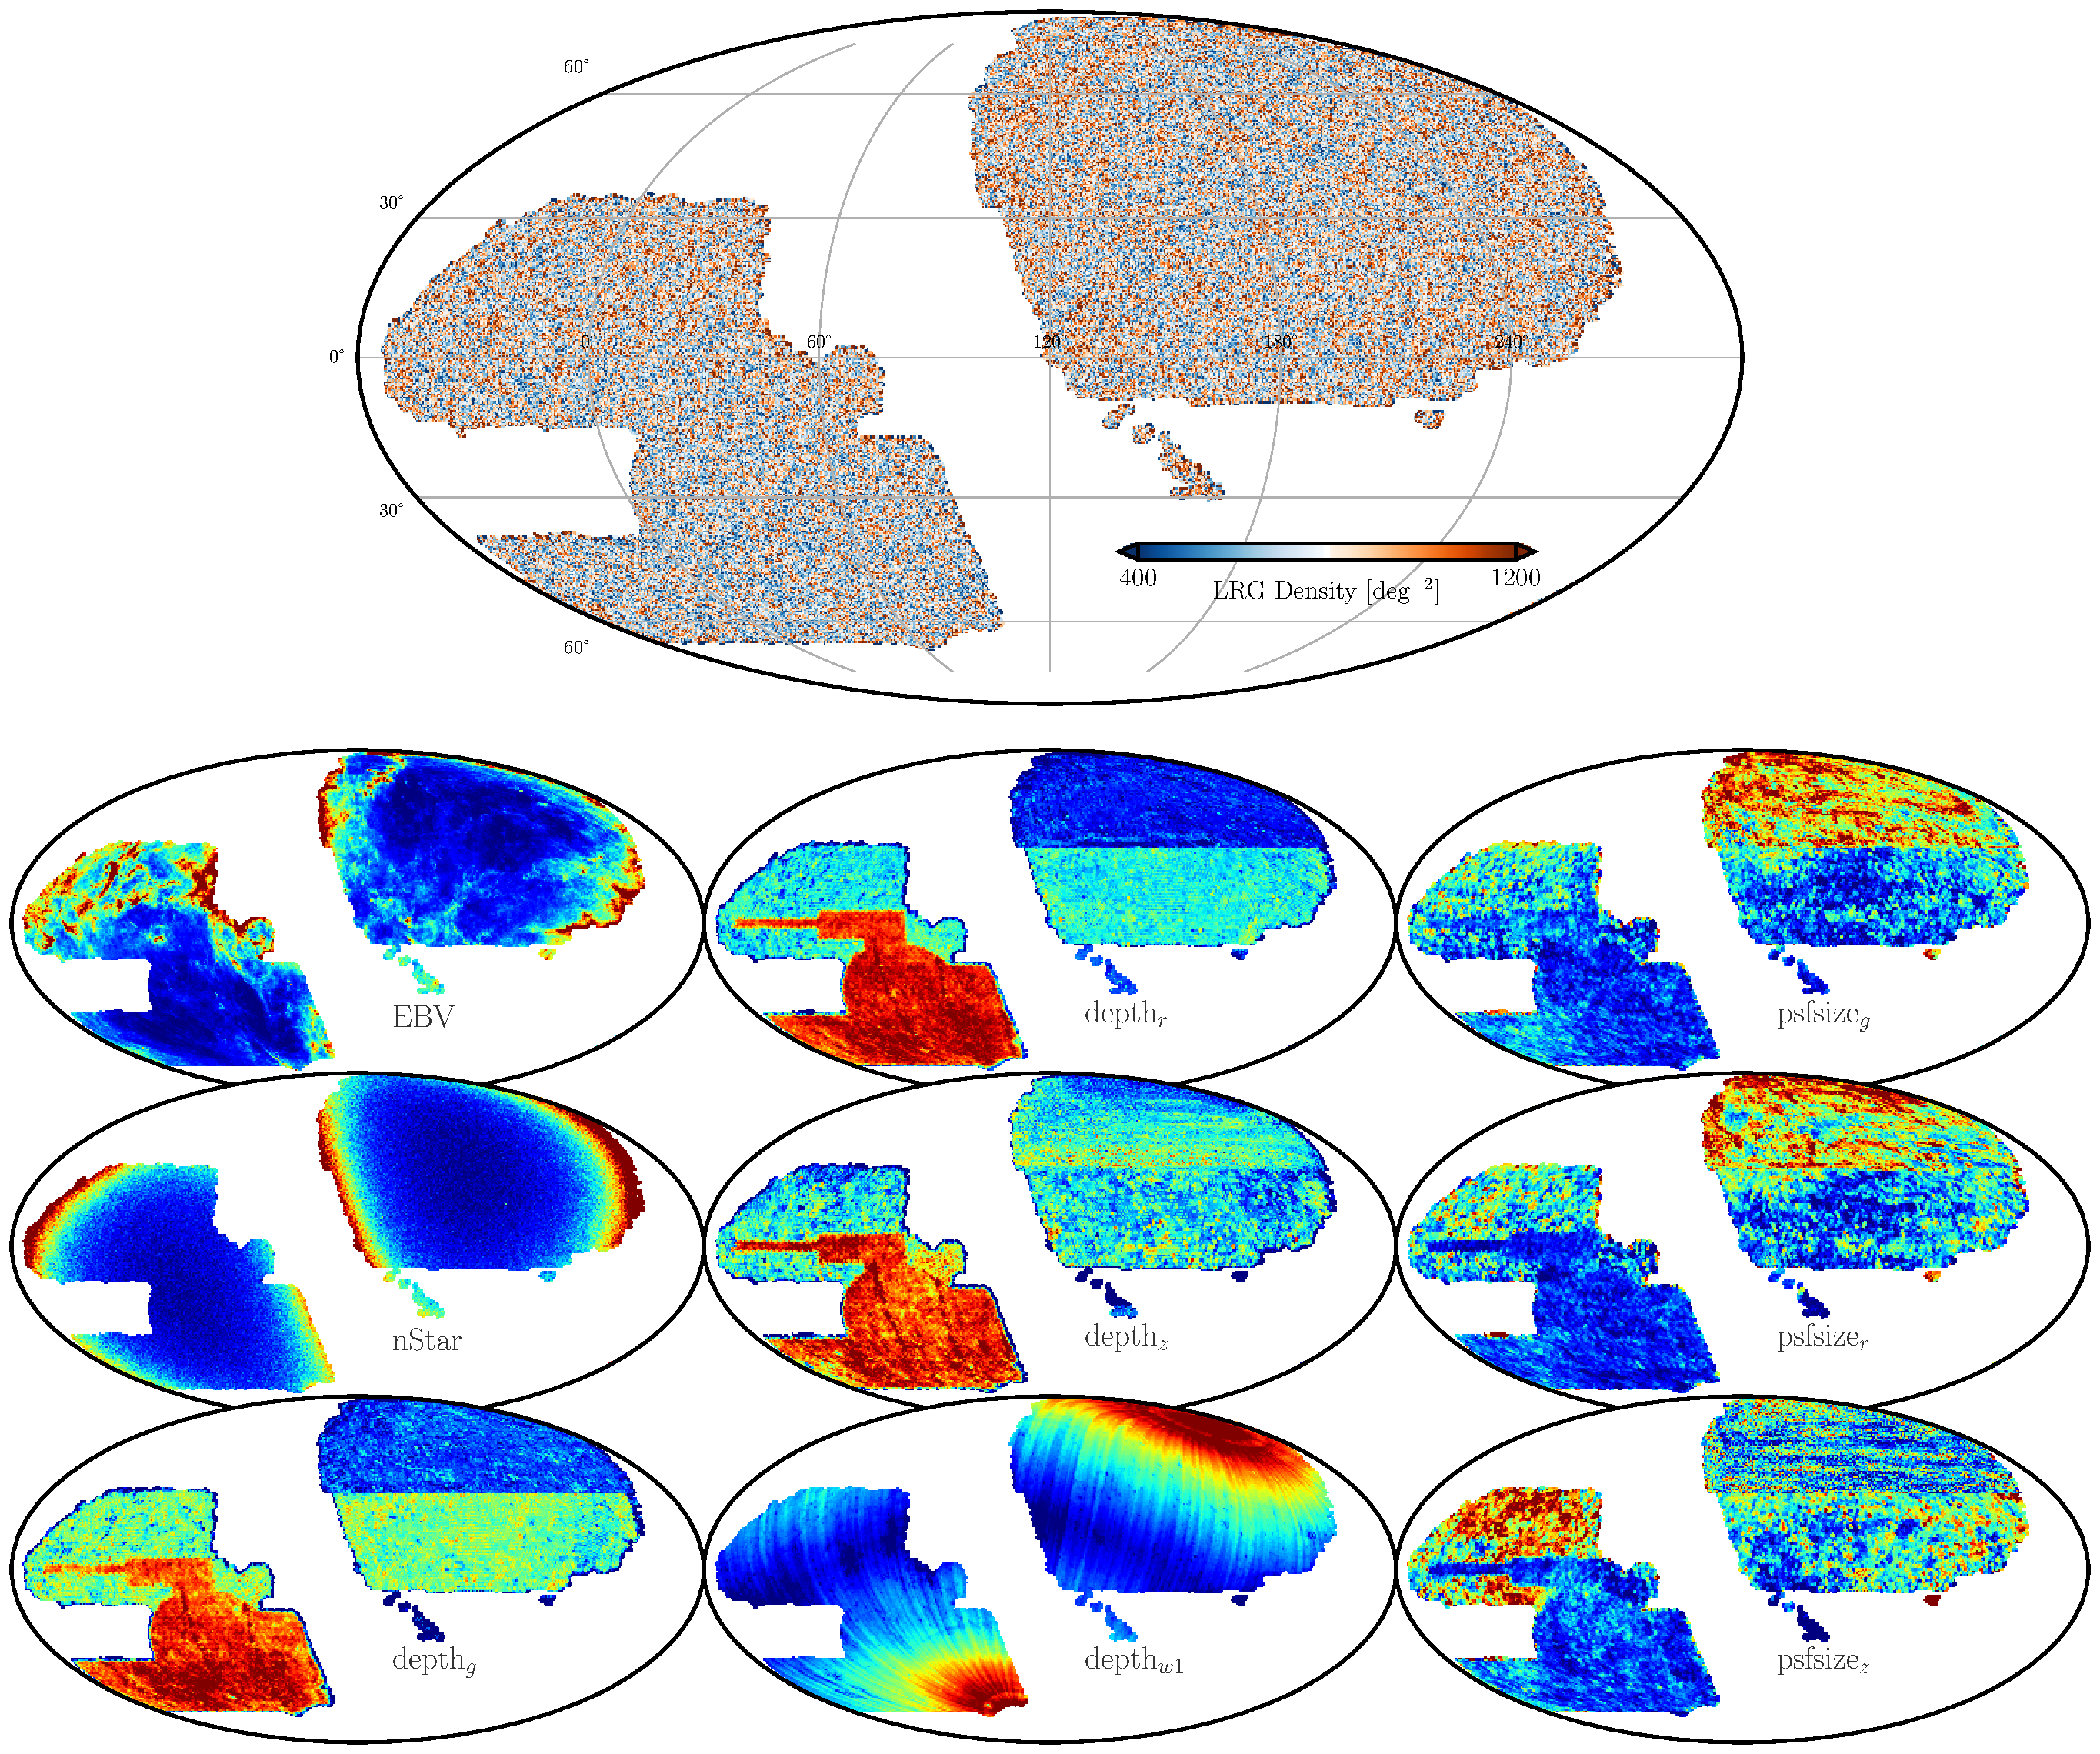
\includegraphics[width=0.99\textwidth]{figures/dr9data.pdf}
 \caption{Top: The DESI LRG target density map before imaging systematics correction in Mollweide projection. Spurious disconnected islands from the North footprint and declination below $-30$ from the South footprint are removed for the analysis due to potential calibration issues (see text). Bottom: Mollweide projections of the DESI DR9 imaging properties (survey depth and astronomical seeing/psfsize) and Milky Way foregrounds (extinction and local stellar density) in celestial coordinates. Two external imaging systematic maps are neutral hydrogen column density and photometric calibration maps (not shown), which are only used for robustness tests. The imaging values are colour-coded to increase from blue to red.}
 \label{fig:ng}
\end{figure*}

The LRG sample is masked rigorously for foreground bright stars, bright galaxies, and clusters of galaxies\footnote{See \url{https://www.legacysurvey.org/dr9/bitmasks/} for maskbit definitions.} to further reduce stellar contamination \citep{zhou2022target}. Then, the sample is binned into \textsc{HEALPix} \citep{gorski2005healpix} pixels at $\textsc{nside}=256$ to construct the 2D density map (as shown in Figure \ref{fig:ng}). The LRG density is corrected for the pixel incompleteness and lost areas using a catalogue of random points, hereafter referred to as randoms, uniformly scattered over the footprint with the same cuts and masks applied. The LRG density map exhibits some large-scale spurious fluctuations, even though that DESI-like LRGs are selected brighter than the imaging survey depth limits. Specifically, the SGC footprint exhibits some systematic under-density while there is some systematic over-density near the survey boundaries in the NGC.

\subsubsection{Imaging systematics}
In this paper, various imaging properties, which can be considered as potential sources of systematic error, are mapped into \textsc{HEALPix} of \textsc{nside}$=256$ (Figure \ref{fig:ng}). The maps include local stellar density constructed from point-like sources with a G-band magnitude in the range $12 \leq G < 17$ from the Gaia DR2 \citep[see,][]{gaiadr2, myers2022}; Galactic extinction E[B-V] from \cite{schlegel1998maps}; survey depth (galaxy depth in $g$, $r$, and $z$ and PSF depth in W1) and astronomical seeing (psfsize) in $g$, $r$, and $z$. These maps have been previously identified as potential sources of imaging systematics in DESI-like LRGs \citep{zhou2022target}. We also consider two external maps for the neutral hydrogen column density (HI) from \cite{2016A&A...594A.116H} and photometric calibration in the z-band (CALIBZ) from \mr{CITE} for robustness tests. %In addition to these sets of imaging systematic maps, we also explore including three extra maps for local stellar density (nStar), magnitude calibration in the z band (CALIBZ), and neural hydrogen column density (HI).

Each imaging map carries its characteristic fluctuations, which correlate with the LRG density map. For instance, large-scale fluctuations can be associated with stellar density, extinction, or survey depth; while small scale-fluctuations can be related to psfsize variations. Upon visual inspection, the under-dense regions of LRGs in the SGC can be associated with varying survey depth, while the over-dense regions in the NGC can be connected to galactic dust or extinction. Some regions of the DR9 footprint are removed from our analysis to avoid potential photometric calibration issues. Some of these regions are disconnected from the main footprint (e.g., spurious islands in the NGC) or different catalogues of standard stars were used for their calibration (DEC$<-30$ in the SGC). The potential impact of these declination cuts on our $\fnl$ constraints is explored in Section \ref{sec:results}. 

\begin{figure}
\centering
 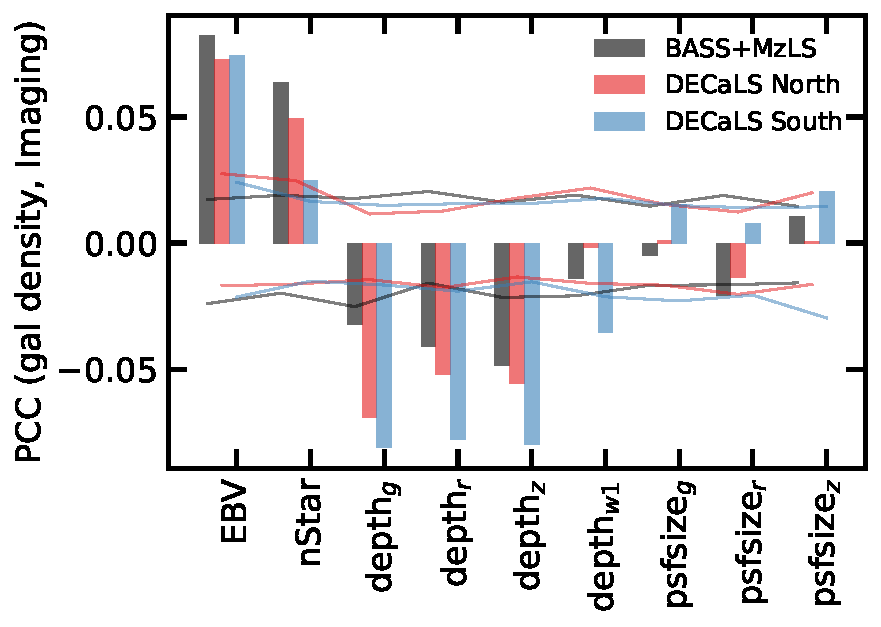
\includegraphics[width=0.45\textwidth]{figures/pcc.pdf} 
 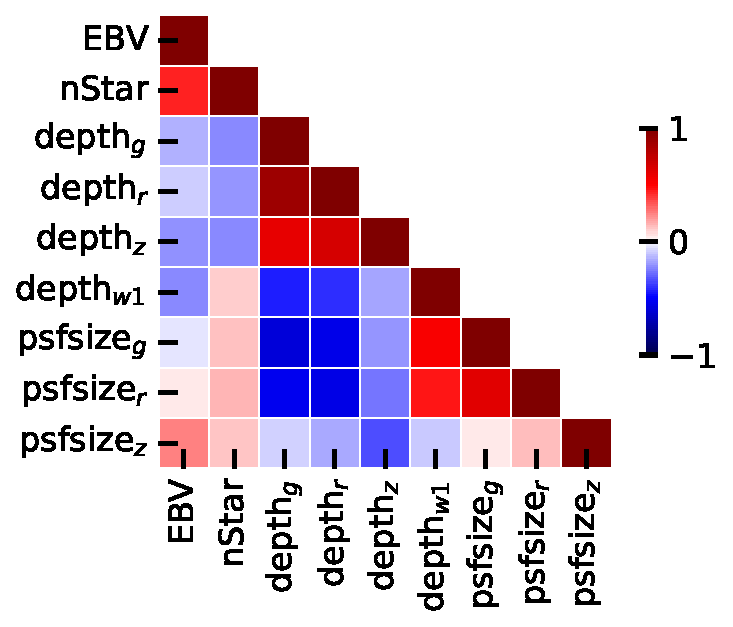
\includegraphics[width=0.45\textwidth]{figures/pccx.pdf}  
 \caption{Top: The Pearson correlation coefficient between the DESI LRG target density and imaging properties in BASS+MzLS, DECaLS North, and DECaLS South. Solid horizontal curves represent the $95\%$ confidence regions estimated from 100 simulated lognormal density maps. Bottom: The Pearson correlation matrix of imaging properties for the DESI footprint.}
 \label{fig:pcc}
\end{figure}

Figure \ref{fig:pcc} shows the Pearson correlation coefficient between the DESI LRG target density and the imaging systematics maps for the three imaging regions (DECaLS North, DECaLS South, and BASS+MzLS) in the top panel. The horizontal curves represent the $95\%$ confidence regions and are constructed by cross-correlating 100 synthetic lognormal density fields and the imaging systematic maps. Figure \ref{fig:pcc} (bottom panel) shows the correlation matrix among the imaging systematics maps for the DESI footprint. There are statistically significant correlations between the LRG density and depth, extinction, and stellar density. There are no significant correlations between the LRG density and the $W1$-band depth and psfsize. Significant inner correlations exist among the imaging systematic maps themselves, especially between the local stellar density and Galactic extinction; also, the $r$-band and $g$-band survey properties are more correlated with each other than with the $z$-band. The Spearman-r correlation coefficient is also applied to measure the relationship between the DESI target density and imaging systematic maps, but no significant differences between the Spearman and Pearson results are found.

The effects of observational systematics in the DESI targets have been studied in great detail \cite[see, e.g.,][]{kitanidis2020imaging, zhou2021clustering, chaussidon2022angular}. There are several approaches for handling imaging systematic errors, broadly classified into data-driven and simulation-based modeling approaches. The general idea behind these approaches is to use the available data or simulations to learn or forward model the relationship between the observed target density and the imaging systematic maps, and to use this relationship, which is often described by a set of \textit{imaging weights}, to correct for systematic errors. Another techniques for reducing the effect of imaging systematics rely on cross-correlating different tracers of dark matter to reduce excess clustering signals, as each tracer might respond differently to a source of systematic error \citep[see, e.g.,][]{giannantonio2014improved}. These methods have their limitations and strengths \citep[see, e.g.,][for a review]{2021MNRAS.503.5061W}.

In this paper, data-driven approaches, including linear multivariate regression and artificial neural networks, are applied to the data to correct for imaging systematic effects. One potential problem that can arise in the data-driven mitigation approach is \textit{over-correction}, which occurs when the corrections applied to the data are too strong that remove the clustering signal and induce additional biases in the inferred parameter. These effects are identified to be of negligible impact on observables like BAO and RSD \citep{merz2021clustering}; however, they can significantly modulate the galaxy power spectrum on large scales, and thus lead to biased $\fnl$ constraints \citep{rezaie2021primordial, mueller2022primordial}. \mr{Although not investigated statistically, these issues could limit the detectability of primordial features in the galaxy power spectrum and that of parity violations in higher order clustering statistics \citep{beutler2019primordial, cahn2021test, philcox2022probing}}. The other challenge is the significant correlations among the imaging systematic maps, as illustrated in the bottom panel of Figure \ref{fig:pcc}. Using highly correlated imaging systematic maps increases the input noise to regression and the potential for over correction. It is crucial to develop, implement, and apply machine learning techniques to control over-correction by reducing the dimensionality of the problem, in the hope of ensuring that the constraints are as accurate and reliable as possible. Our goal is to reduce the correlations between the LRG target density and the imaging systematic maps, while minimizing over correction. To achieve this, we employ a statistical method that involves identifying different sets of the imaging systematic maps using cross power spectrum, mean galaxy density statistics, and simulations which we will present later in Section \ref{sec:method}: 
\begin{enumerate}[itemindent=*]
\item \textbf{Two maps}: Extinction, depth in z.
\item \textbf{Three maps}: Extinction, depth in z, psfsize in r.
\item \textbf{Four maps}: Extinction, depth in z, psfsize in r, stellar density.
\item \textbf{Five maps}: Extinction, depth in z, psfsize in r, neutral hydrogen density, and calibration in z.
\item \textbf{Eight maps}: Extinction, depth in $grzW1$, psfsize in $grz$.
\item \textbf{Nine maps}: Extinction, depth in $grzW1$, psfsize in $grz$, stellar density.
\end{enumerate}
 
Both linear and neural network models are trained on each imaging region separately since the Pearson correlation coefficient analysis indicated each region responds differently to the imaging systematic maps, as illustrated in the top panel of Figure \ref{fig:pcc}. The linear multivariate model only uses the imaging systematic maps up to the linear power. With this model, the predicted number counts of targets in pixel $i$ is given by
\begin{equation}\label{eq:npred}
    \rho_{i} = \log ( 1 + \exp[\textbf{a}.\textbf{x}_{i}]),
\end{equation}
where $\textbf{a}.\textbf{x}_{i}$ represents the inner product between the parameters, $\textbf{a}$, and imaging systematic values for pixel $i$, $\textbf{x}_{i}$. The implementation of Markov Chain Monte Carlo (MCMC) random search from \textsc{emcee} \citep{2013PASP..125..306F} is used to explore the parameter space by minimizing the negative Poisson log-likelihood between the actual and predicted number counts of targets. No spatial coordinates is included in $\textbf{x}_{i}$ to help avoid over correction, and as a result, the predicted number counts solely reflect the spurious density fluctuations that arise from varying imaging conditions. The number of pixels is substantially larger than the number of parameters for the linear model, and thus no training-validation-testing split is applied to the data. This aligns with the methodology used for training linear models in previous analyses \citep[see, e.g.,][]{zhou2022target}. The marginalized mean of the parameters are then utilized to compute imaging weights are then defined as the

Our neural network-based mitigation approach uses the implementation of fully connected feedforward neural networks from \cite{rezaie2021primordial}. With the neural network approach, $\textbf{a}.\textbf{x}_{i}$ in Equation \ref{eq:npred} is replaced with $NN(\textbf{x}_{i}|\textbf{a})$, where $NN$ represents the fully connected neural network and $\textbf{a}$ being its parameters. The application of these neural networks on galaxy survey data is explained in detail in \cite{rezaie2021primordial}, including their implementation, training, and validation. This information will be briefly summarized here. 

A fully connected feedforward neural network (also called a \textit{multi-layer perceptron}) is a type of artificial neural network where the neurons are arranged in layers, and each neuron in one layer is connected to every neuron in the next layer. The imaging systematic information flows only in one direction, from input to output. Each neuron applies a nonlinear activation function (i.e., transformation) to the weighted sum of its inputs, which are the outputs of the neurons in the previous layer. The output of the last layer is the prediction of the model for the number counts of galaxies. Our architecture consists of three hidden layers with 20 rectifier activation functions on each layer, and a single neuron in the output layer. The rectifier is defined as ${\rm max}(0, x)$ \citep{nair2010rectified}. This simple form of nonlinearity is very effective in enabling deep neural networks to learn more complex, nonlinear relationships between the input imaging maps and output galaxy counts.

Unlike linear regression, neural networks are prone to fitting noise, i.e., excellent performance on training data and poor performance on unseen data. Therefore, our analysis uses a training-validation-testing split to ensure that the network is well-optimized and generalizes well to unseen data. Specifically, $60\%$ of the LRG data is used for training, $20\%$ is used for validation, and $20\%$ is used for testing. The neural network models are tested on the entirety of the LRG sample with the technique of permuting the choice of the training, validation, or testing sets \citep{arlot2010survey}. The neural networks are trained for up to 70 training epochs with the gradient descent \textsc{Adam} optimizer \citep{2017arXiv171105101L}. The neural network parameters are adjusted iteratively following the gradient of the negative Poisson log-likelihood. The step size of the parameter updates is controlled via the learning rate hyper-parameter, which is initialized with a grid search and is designed to dynamically vary between two boundary values of $0.001$ and $0.1$ to avoid local minima \citep[see, also,][]{2016arXiv160803983L}. At each training epoch, the neural network model is applied to the validation set, and ultimately the model with the best performance on validation is identified and applied to the test set. With the cross-validation technique, the model predictions from the different test sets are aggregated together to form the predicted target density map into \textsc{HEALPix} of \textsc{nside} $=256$. To reduce the error in the predicted number counts, we train an ensemble of 20 neural network models and average over the predictions. The imaging weights are then defined as the inverse of the predicted target density, normalized to unity.

A visual inspection of the predicted target density maps reveals that most of the large-scale spurious fluctuations are explained by just extinction and depth in the z-band. Adding psfsize in the r-band results in more small-scale spurious fluctuations in the predicted target density maps. Our inspection shows that using all of the imaging systematic maps as input for regression does not provide more information, which is expected from highly correlated predictors (Figure \ref{fig:pcc}). Given the same set of inputs, the neural network-based weights show more small-scale spurious fluctuations which can be associated with the higher flexibility of the underlying model. Both approaches yield large-scale spurious fluctuations consistent with the LRG target density; for instance, both models predict a higher density of LRGs near the boundaries where the DESI imaging surveys observed regions of high extinction or high stellar density near the galactic plane. These over-dense regions are likely contaminated artifacts entering the LRG selection, e.g., stellar contaminants or other artifacts because of obscured photometry from extinction. This is interesting since the target selection cuts use extinction corrected magnitudes. Further robustness tests on these weights are discussed in Section \ref{sec:method}, and their impacts on $\fnl$ are presented in Section \ref{sec:results}.


\subsection{Synthetic lognormal density fields}\label{ssec:mocks}
Density fluctuations of galaxies on large scales can be approximated with lognormal distributions \citep{coles1991}. Unlike N-body simulations, simulating lognormal density fields is not computationally intensive, and allows quick and robust validation of data analysis pipelines. These mocks are therefore considered useful for our study since the signature of local PNG appears on large-scales and small scale clustering is not used. The package \textsc{FLASK} \citep[Full-sky Lognormal Astro-fields Simulation Kit;][]{Xavier_2016} is employed to generate ensembles of synthetic lognormal density maps that mimic the redshift and angular distributions of the DR9 LRG targets. Two universes with $\fnl=0$ and $76.92$ are considered. A set of 1000 realizations are produced for every $\fnl$. The bias is assumed to vary with redshift by $b(z)=1.43/D(z)$, where $D(z)$ denotes the growth factor \citep[see, e.g.,][]{zhou2021clustering}. With this bias evolution, the clustering amplitude remains constant. The analysis adapts a fiducial cosmology from a flat $\Lambda$CDM universe, including one massive neutrino with $m_{\nu}=0.06$ eV, Hubble constant $h = 0.67$, matter density $\Omega_{M}=0.31$, baryon density $\Omega_{b}=0.05$, and spectral index $n_{s}=0.967$. The amplitude of the matter power spectrum on a scale of $8, h^{-1} \text{Mpc}$ is set as $\sigma_{8}=0.8225$. The same fiducial cosmology is used throughout this paper unless specified otherwise. \mr{The robustness of our constraints against the fiducial cosmology is explored in Section \ref{sec:results}.}

\subsubsection{Contaminated mocks}
The linear model is employed to introduce synthetic spurious fluctuations in the lognormal density fields. The motivation for choosing a linear contamination model is to assess how much of the clustering signal can be removed by applying more flexible and rigorous models, based on neural networks, for correcting imaging systematic effects. The parameter space of the linear model is explored using MCMC, from the relationship between the DESI LRG target sample and the imaging systematic maps. The MCMC process is executed separately on each imaging survey using only \textit{three maps} (extinction, depth in z, and psfsize in r) as $\textbf{x}_{i}$. The imaging selection function for contaminating each simulation is uniquely and randomly drawn from the parameter space probed by MCMC, and then the results from each imaging survey are combined to form the DESI footprint. The same contamination model is used for both the $\fnl=0$ and $76.92$ simulations.

Similar to the imaging systematic treatment analysis for the DESI LRG targets, the neural network methods with various combinations of the imaging systematic maps are applied to each simulation, with and without PNG, and with and without systematics, to derive the imaging weights. Section \ref{sec:method} presents how the simulation results are incorporated to calibrate $\fnl$ biases due to over-correction. 